\documentclass{article}

\usepackage{fancyhdr}
\usepackage{extramarks}
\usepackage{amsmath}
\usepackage{amsthm}
\usepackage{amssymb}
\usepackage{amsfonts}
\usepackage{tikz}
\usepackage{physics}
\usepackage[plain]{algorithm}
\usepackage{algpseudocode}
\usepackage{hyperref}

\usetikzlibrary{automata,positioning}

%
% Basic Document Settings
%

\topmargin=-0.45in
\evensidemargin=0in
\oddsidemargin=0in
\textwidth=6.5in
\textheight=9.0in
\headsep=0.25in

\linespread{1.1}

\pagestyle{fancy}
\lhead{\hmwkAuthorName}
\chead{\hmwkClass\ : \hmwkTitle}
\rhead{\firstxmark}
\lfoot{\lastxmark}
\cfoot{\thepage}

\renewcommand\headrulewidth{0.4pt}
\renewcommand\footrulewidth{0.4pt}

\setlength\parindent{0pt}

%
% Create Problem Sections
%
\newcommand{\be}{\begin{equation}}
\newcommand{\ee}{\end{equation}}
\newcommand{\bes}{\begin{equation*}}
\newcommand{\ees}{\end{equation*}}
\newcommand{\bea}{\begin{flalign*}}
\newcommand{\eea}{\end{flalign*}}


\newcommand{\enterProblemHeader}[1]{
    \nobreak\extramarks{}{Problem \arabic{#1} continued on next page\ldots}\nobreak{}
    \nobreak\extramarks{Problem \arabic{#1} (continued)}{Problem \arabic{#1} continued on next page\ldots}\nobreak{}
}

\newcommand{\exitProblemHeader}[1]{
    \nobreak\extramarks{Problem \arabic{#1} (continued)}{Problem \arabic{#1} continued on next page\ldots}\nobreak{}
    \stepcounter{#1}
    \nobreak\extramarks{Problem \arabic{#1}}{}\nobreak{}
}

\setcounter{secnumdepth}{0}
\newcounter{partCounter}
\newcounter{homeworkProblemCounter}
\setcounter{homeworkProblemCounter}{1}
\nobreak\extramarks{Problem \arabic{homeworkProblemCounter}}{}\nobreak{}

%
% Homework Problem Environment
%
% This environment takes an optional argument. When given, it will adjust the
% problem counter. This is useful for when the problems given for your
% assignment aren't sequential. See the last 3 problems of this template for an
% example.
%
\newenvironment{homeworkProblem}[1][-1]{
    \ifnum#1>0
        \setcounter{homeworkProblemCounter}{#1}
    \fi
    \section{Problem \arabic{homeworkProblemCounter}}
    \setcounter{partCounter}{1}
    \enterProblemHeader{homeworkProblemCounter}
}{
    \exitProblemHeader{homeworkProblemCounter}
}

%
% Homework Details
%   - Title
%   - Due date
%   - Class
%   - Section/Time
%   - Instructor
%   - Author
%

\newcommand{\hmwkTitle}{Assignment\ \#1}
\newcommand{\hmwkDueDate}{Due on 18th January, 2019}
\newcommand{\hmwkClass}{Advanced Statistical Mechanics}
\newcommand{\hmwkClassTime}{}
\newcommand{\hmwkClassInstructor}{}
\newcommand{\hmwkAuthorName}{\textbf{Aditya Vijaykumar}}

%
% Title Page
%

\title{
    %\vspace{2in}
    \textmd{\textbf{\hmwkClass:\ \hmwkTitle}}\\
    \normalsize\vspace{0.1in}\small{\hmwkDueDate\ }\\
%    \vspace{3in}
}

\author{\hmwkAuthorName}
\date{}

\renewcommand{\part}[1]{\textbf{\large Part \Alph{partCounter}}\stepcounter{partCounter}\\}

%
% Various Helper Commands
%

% Useful for algorithms
\newcommand{\alg}[1]{\textsc{\bfseries \footnotesize #1}}

% For derivatives
\newcommand{\deriv}[1]{\frac{\mathrm{d}}{\mathrm{d}x} (#1)}

% For partial derivatives
\newcommand{\pderiv}[2]{\frac{\partial}{\partial #1} (#2)}

% Integral dx
\newcommand{\dx}{\mathrm{d}x}

% Alias for the Solution section header
\newcommand{\solution}{\textbf{\large Solution}}

% Probability commands: Expectation, Variance, Covariance, Bias
\newcommand{\E}{\mathrm{E}}
\newcommand{\Var}{\mathrm{Var}}
\newcommand{\Cov}{\mathrm{Cov}}
\newcommand{\Bias}{\mathrm{Bias}}

\begin{document}

\maketitle
(\textbf{Acknowledgements} - I would like to thank Aditya Sharma and Junaid Majeed for discussions.)

\begin{homeworkProblem}[1]
	\textbf{Part (a)}\\
	Given that 
	\begin{align*}
	X &= \dfrac{\sum_{i=1}^N X_i}{\sigma \sqrt{N}} \\
	\ev{X} &= \dfrac{\sum_{i=1}^N \ev{X_i}}{\sigma \sqrt{N}} = \dfrac{\sum_{i=1}^N 0}{\sigma \sqrt{N}} = 0\\
	\sqrt{\ev{X^2}} &= \dfrac{\sqrt{\sum_{i=1}^N \sum_{j=1}^N \ev{X_i X_j}}}{\sigma \sqrt{N}} \\ 
	&=  \dfrac{\sqrt{\sum_{i=1}^N \sum_{j=1}^N \ev{X_i^2} \delta_{ij}}}{\sigma \sqrt{N}} \impliedby \qq{independent variables, hence covariance is zero}\\
	&= \dfrac{\sqrt{\sum_{i=1}^N\sigma^2 }}{\sigma \sqrt{N}}\\
	\sigma_X &= \dfrac{\sqrt{N \sigma^2 }}{\sigma \sqrt{N}} = 1
	\end{align*}
	
	\textbf{Part (b)}\\
	Let $ x, y - x, 1- y $ be the lengths of the 3 sticks after breaking. Triangle inequality gives us the following conditions on the stick,
	\begin{align*}
	x < 1-x \implies x < \dfrac{1}{2}\\
	y - x < x + 1 - y \implies y -x > \dfrac{1}{2}\\
	1-y < y \implies y > \dfrac{1}{2}
	\end{align*}
	In the unit square of the $ x-y $ plane, we need to find the intersection of the above regions. The first and last regions have an intersection of are$ \dfrac{1}{4} $ in the plane, and the second region automatically includes this intersection. Hence the required probability is $ \dfrac{1}{4}$.
	
	
	\textbf{Part (c)}\\
	The histograms are plotted below,
	\begin{figure}[!h]
		\centering
		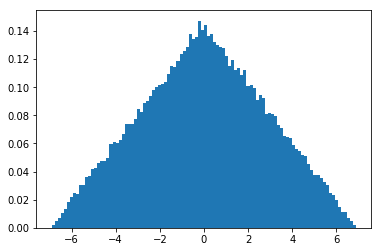
\includegraphics[scale=0.5]{trace_u.png}
		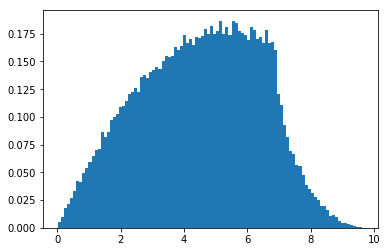
\includegraphics[scale=0.5]{d.png}
		\caption{L : Trace Distribution, R: Eigenvalue Spacing Distribution for Uniform case}
	\end{figure}

	\begin{figure}[!h]
		\centering
		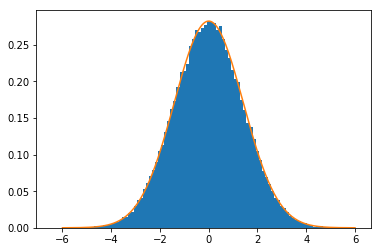
\includegraphics[scale=0.5]{distr_n.png}
		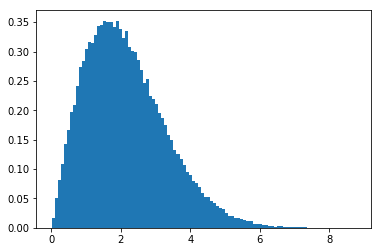
\includegraphics[scale=0.5]{trace_n.png}
		\caption{L : Trace Distribution, R: Eigenvalue Spacing Distribution for Normal case}
	\end{figure}


	\textbf{Part (d)}\\
	In our case, in time interval $ dt $, the walker can go left with probability $ \alpha dt$, right with probability $ \alpha dt$ and can stay at the same position with probability $ 1 - 2 \alpha dt $. So then, at position $ i $ and time $ t + dt $,
	\begin{align*}
	P(i, t + dt) &= P(i,t) (1 - 2 \alpha dt) + (P(i+1,t) + P(i-1,t)) \alpha dt\\
	\pdv{P(i, t)}{t} &= - 2 P(i,t) \alpha   + (P(i+1,t) + P(i-1,t)) \alpha \\
	\end{align*}
	We solve the above equation by writing down the Fourier series. Every step away from $ i $th site will introduce factors of $ e^{jk} $ in the Fourier space,
	\begin{align*}
	\pdv{P(k,t)}{t} &= (-2 \alpha + e^{jk} + e^{-jk}) P(k,t)
	\end{align*}
	We know that $ P(x,t=0) = \delta_{x,0} \implies P(k,t=0) = 1   $ and then the solution to the above equation is,
	\begin{align*}
	P(k,t) &= e^{ (-2 \alpha + e^{jk} + e^{-jk})t}\\
	&= e^{- 2 \alpha t} \sum_{x=-\infty}^{\infty } e^{2jkx \cos k}\\
	P(k,t)&= e^{- 2 \alpha t} \sum_{x=-\infty}^{\infty } e^{2jkx} I_x(t)
	\end{align*}
	From which we can see by inverse Fourier,  $ P(x,t) =  e^{- 2 \alpha t} I_x(t) $, where $ I_x(t) $ is the Bessel function of the first kind.	
	
	\textbf{Part (e)}\\
	Let's say the random walker takes $ x $ steps rightward and $ y $ steps leftward. For this walker to be at $ r $ after $ N $ steps, $ x + y = N $ and $ x-y = r $ $ \implies x = \dfrac{N+r}{2} $ and $ y = \dfrac{N - r}{2} $. The probability $ P(r,N) $ is then,
	\begin{align*}
	P(r,N) &= {N \choose r} \dfrac{1}{2^{x}} \dfrac{1}{2^{y}} \\
	&= {N \choose x} \dfrac{1}{2^{N}}
	\end{align*} 
	
	For very large $ N $,
	\begin{align*}
	{n \choose x} = \dfrac{N!}{x! y!} &= \dfrac{N!}{\qty(\dfrac{N+r}{2})!\qty(\dfrac{N-r}{2})!}\\
	&=\dfrac{e^{-N} N^N}{(N+r)^{(N+r)/2} (N-r)^{(N-r)/2} 2^{-N} e^{-N}}\\
	&= \dfrac{N^N}{(1+r/N)^{(N+r)/2} (1-r/N)^{(N-r)/2} 2^{-N} N^N }\\
	P(r,N) &= \dfrac{1}{(1+r/N)^{(N+r)/2} (1-r/N)^{(N-r)/2}}\\
	P(r,N) &= [{(1+r/N)^{(1+r/N)} (1-r/N)^{(1-r/N)}}]^{-N/2}
	\end{align*}
	Comparing with the form $ P(r,N) = e^{-N \phi(r/N)} $, we get,
	\begin{equation*}
	\phi(x) =\dfrac{ (1+x) \ln (1+x) + (1 -x ) \ln (1-x)}{2}
	\end{equation*}
	
\end{homeworkProblem}







\begin{homeworkProblem}[2]
	\textbf{Part (a)}\\
	For constant number of particles, 
	\begin{equation*}
	dU = -PdV + TdS + hdM
	\end{equation*}
	The enthalpy $ E $ is defined as $E = U + PV$,
	\begin{align*}
	dE &= dU + PdV + VdP = -PdV + TdS + hdM + PdV + VdP \\
	&=  TdS + hdM  + VdP
	\end{align*}
	The Helmholtz Potential $ A $ is defined as $A = U - TS$,
	\begin{align*}
	dA &= dU - TdS - SdT  = -PdV + TdS + hdM - TdS - SdT  \\
	&= -PdV + hdM  - SdT 
	\end{align*}
	The Gibbs Potential $ G = E - TS $, 
	\begin{align*}
	dG &=  TdS + hdM  + VdP - TdS - SdT\\
	&=   hdM  + VdP - SdT
	\end{align*}
	As all the quantities are related by Legendre Transforms, knowledge of one of the quantities is enough to calculate all the others.
	
	\textbf{Part (b)}\\
	$ C_x $ and $ \kappa_x $ are defined as follows,
	\begin{equation*}
	C_x = \eval{\dv{Q}{T}}_{x = const.} \qq{} \kappa_x = -\eval{\dfrac{1}{V}\dv{V}{P}}_{x = const.}
	\end{equation*}
	Consider the following,
	\begin{align*}
	C_P = T \eval{\dv{S}{T}}_{P = const} = -T \pdv[2]{G}{T} \implies \pdv[2]{G}{T} < 0 \implies G(T) \text{ is concave}\\
	C_V = T \eval{\dv{S}{T}}_{V = const} = -T \pdv[2]{A}{T} \implies \pdv[2]{A}{T} < 0 \implies A(T) \text{ is concave}\\
	\kappa_T = -\eval{\dfrac{1}{V}\dv{V}{P}}_{T = const.} = -\dfrac{1}{V} \pdv[2]{G}{P} \implies \pdv[2]{G}{P} < 0 \implies G(P) \text{ is concave}\\
	\kappa_T = -\eval{\dfrac{1}{V}\dv{V}{P}}_{T = const.} = \dfrac{1}{V} \dfrac{1}{\pdv[2]{A}{V} }\implies \pdv[2]{A}{V} > 0 \implies A(V) \text{ is convex}\\
	\end{align*}
\end{homeworkProblem}









\begin{homeworkProblem}[3]
	Given $ S_{Gibbs} = - \sum_a p_\alpha \log p_\alpha $, which we have to maximize under $ \sum_\alpha p_\alpha = 1 $. We use the method of Lagrange multipliers, $ f(p_\alpha) = - \sum_a p_\alpha \log p_\alpha + \lambda (\sum_\alpha p_\alpha - 1) $,
	\begin{align*}
	\dv{f}{p_\gamma} &= - \log p_\gamma - 1 + \lambda = 0 \\
	\implies \lambda &= 1 + \log p_\gamma \implies p_\gamma = constant = \dfrac{1}{N} 
	\end{align*}
	where $ N $ is the number of microstates. Hence, we have shown that the all microstates are equally likely in microcanonical ensemble.
	
	Similarly, we proceed to carry out the calculation for canonical ensemble and grand canonical ensemble. In this case, $ f(p_\alpha) = - \sum_a p_\alpha \log p_\alpha + \lambda_1 (\sum_\alpha p_\alpha - 1) +  \lambda_2 (\sum_\alpha p_\alpha E_\alpha - \ev{E}) $,
	\begin{align*}
	\dv{f}{p_\gamma} &= - \log p_\gamma - 1 + \lambda_1 + \lambda_2 E_\gamma = 0\\
	\implies p_\gamma &= \exp(\lambda_1 - 1) \exp(\lambda_2 E_\gamma)
	\end{align*}
	which is the expression for probability in the canonical ensemble \textit{ie}. some normalization times $ \exp(\beta E_\gamma) $.
	
	For the grand canonical ensemble, $ f(p_\alpha) = - \sum_a p_\alpha \log p_\alpha + \lambda_1 (\sum_\alpha p_\alpha - 1) +  \lambda_2 \qty(\sum_\alpha p_\alpha E_\alpha - \ev{E}) +\lambda_3 (\sum_\alpha N_\alpha p_\alpha - \ev{N})$,
	\begin{align*}
	\dv{f}{p_\gamma} &= - \log p_\gamma - 1 + \lambda_1 + \lambda_2 E_\gamma + \lambda_3 N_\gamma = 0\\
	\implies p_\gamma &= \exp(\lambda_1 - 1) \exp(\lambda_2 E_\gamma + \lambda_3 N_\gamma)
	\end{align*}
	which is the expression for probability in the canonical ensemble \textit{ie}. some normalization times $ \exp(\beta E_\gamma + \mu N_\gamma) $.
	
	\textbf{Part (b)}\\
	We first write down the partition function for a classical ideal gas,
	\begin{align*}
	Z &= \dfrac{1}{h^{3N} N!} \prod_{i=1}^{N} \int d^3q_i d^3 p_i \exp(-\beta p_i^2/2m)\\
	&= \dfrac{1}{h^{3N} N!} \prod_{i=1}^{N} V \qty(\dfrac{2 \pi m}{\beta})^{3/2}\\
	&= \dfrac{ V^N}{h^{3N} N!} \qty(\dfrac{2 \pi m}{\beta})^{3N/2}
	\end{align*}
	
	So then, the probability is given by,
	\begin{align*}
	P(N=N) &= \sum_{\epsilon_i} \dfrac{e^{\beta \mu N} e^{-\beta \epsilon_i}}{Z}\\
	&= \dfrac{e^{\beta \mu N}}{e^{\ev{N}}} \dfrac{1}{N!} \qty(\dfrac{V}{\lambda^3})^N\\
	&= \dfrac{e^{-\ev{N}} \ev{N}^N}{N!}
	\end{align*}
\end{homeworkProblem}







\begin{homeworkProblem}[4]
	\begin{align*}
	f_\nu (z ) &= \dfrac{1}{\Gamma(\nu)} \int_{0}^{\infty}  \dd x \dfrac{x^{\nu - 1}}{z^{-1} e^x + 1}\\
	&= \dfrac{1}{\Gamma(\nu)} \qty[ \eval{\dfrac{x^{\nu}}{\nu(z^{-1} e^x + 1)}}_{0}^{\infty} - \int_{0}^{\infty}  \dd x \dfrac{x^{\nu}}{\nu } \dv{z^{-1} e^x + 1}{x}]\\
	&= -\dfrac{1}{\Gamma(\nu+1)} \qty[ \dd x {x^{\nu}} \dv{z^{-1} e^x + 1}{x}]
 	\end{align*}
 	We change the variables to $ x=  \ln z + t$ and get,
 	\begin{align*}
 	f_\nu(z) &\approx -\dfrac{1}{\Gamma(\nu + 1)} \int_{-\infty}^\infty dt (\ln z + t )^\nu \dv{t} \qty(\dfrac{1}{z^{-1} z e^t + 1})\\
 	&\approx -\dfrac{1}{\Gamma(\nu + 1)} \int_{-\infty}^\infty dt \sum_m \dfrac{\nu!}{m! (\nu -m)!} t^m ( \ln z)^{\nu - m}  \dv{t} \qty(\dfrac{1}{e^t + 1})\\
 	&\approx \dfrac{1}{\Gamma(\abs{\nu - m} + 1)} \int_{-\infty}^\infty dt \sum_m ( \beta \mu)^{\nu - m}  I_m
 	\end{align*}
 	
 	\textbf{Part (b)}\\
 	\begin{align*}
 	N &= \dfrac{V}{\lambda^3} f_{3/2} \\
 	&= \dfrac{V}{\lambda^3} \qty(\dfrac{(\beta \mu)^{3/2}}{\Gamma(5/2)}  +  \qty(\dfrac{(\beta \mu)^{-1/2}}{\Gamma(3/2)} 2 f_2^- (1) ))\\
 	&=\dfrac{V \beta^{-3/2}}{(2 \pi m)^{-3/2}} \qty(\dfrac{4\mu^3/2}{3} + 4 \mu^{-1/2} \beta^2 f_2^-(1))\\
 	&= \dfrac{4V \mu^{3/2}}{3 \pi (2 m \pi)^{3/2}} + \dfrac{4 V \mu^{-1/2} \beta f_2(1)}{\pi (2 m \pi )^{3/2}}
 	\end{align*}
 	
 	\begin{align*}
 	E &= \dfrac{3 V (\beta)^{-5/2} }{2 \lambda^3 } f_{5/2}(z)\\
 	&= \dfrac{3V \beta^{-5/2}}{2 (2 \pi m)^{-3/2}} \qty[\dfrac{(\beta \mu)^{5/2}}{\Gamma (7/2)} + \dfrac{(\beta \mu)^{1/2}}{\Gamma (3/2)} (2 f_2^-(1))]\\
 	&= \dfrac{3V }{2 (2 \pi m)^{-3/2}} \qty[\dfrac{(\mu)^{5/2}}{\Gamma (7/2)} + \dfrac{(\beta)^{-2} (\mu)^{1/2}}{\Gamma (3/2)} (2 f_2^-(1))]
 	\end{align*}
 	\begin{equation*}
 	C_V = \lim\limits_{T \rightarrow 0} \pdv{E}{T} = \dfrac{3V \mu^{1/2} (2 \pi m)^{3/2}}{\Gamma(3/2)} k_B^2 T
 	\end{equation*}
\end{homeworkProblem}

















\begin{homeworkProblem}[5]
	\textbf{Part (b)}\\
	We are given,
	\begin{equation*}
	H_N = \sum_{i=1}^N \dfrac{p_i^2}{2m} + \sum_{i=1}^{N-1} u(x_i - x_{i-1}) +v (x_1) + v(x_N)
	\end{equation*}
	One can write the expression of the partition function as follows,
	\begin{align*}
	Z &= \dfrac{1}{N!} \prod_{i}^N \int \int \dfrac{\dd{p_i} \dd{x_i}}{h} \exp(-\beta H_N) \\
	&= \dfrac{1}{N!h^N} \prod_{i}^N \int  \dd{p_i} \exp(-\beta p_i^2/2m) \prod_{i} \int \dd{x_i} \exp(-\beta \sum_{i=1}^{N-1} u(x_i - x_{i-1})  )\\
	&= \dfrac{1}{N!h^N} \qty(\dfrac{2 \pi m}{\beta})^{N/2} \prod_{i} \int \dd{x_i} \exp(-\beta \sum_{i=1}^{N-1} u(x_i - x_{i-1})  )
	\end{align*}
	Consider,
	\begin{align*}
	\prod_{i} \int \dd{x_i} \exp(-\beta \sum_{i=1}^{N-1} u(x_i - x_{i-1})  ) &= \prod_{i \ne 1} \int \dd{x_i} \exp(-\beta \sum_{i=1}^{N-1} u(x_i - x_{i-1})  + v(x_i) ) \int_{-\infty }^\infty \dd x_1 e^{-\beta u(x_2 - x_1) + v(x_1)}\\
	&= \prod_{i \ne 1} \int \dd{x_i} \exp(-\beta \sum_{i=1}^{N-1} u(x_i - x_{i-1})  + v(x_i) ) \int_{a/2 }^{x_2 -a } \dd x_1\\
	&= \prod_{i \ne 1} \int \dd{x_i} \exp(-\beta \sum_{i=1}^{N-1} u(x_i - x_{i-1})  + v(x_i) ) (x_2 - 1.5 a)
	\end{align*}
	We have done one integral, and we now similarly separate out integrals over the other $ x_i $'s. The constant terms will integrate to zero, while the terms involving $ x_i $'s can be simply integrated as power functions. After $ N $ integrals, one will be left with,
	\begin{align*}
	\int_{(N - a/2 )}^{L  - a/2} \dd x_N \dfrac{1}{(N-1)!} \exp(\beta u(x_N - x_{N-1}) - \beta v (x_N)) \qty(x_N - \dfrac{N-1}{2}a)^{N-1}\\
	&= \int_{(N - a/2 )}^{L  - a/2} \dd x_N \dfrac{1}{(N-1)!} \qty(x_N - (N-0.5)a)^{N-1}\\
	&=\dfrac{1}{N!} \qty(L - \dfrac{a}{2} - Na + \dfrac{a}{2})^N\\
	&= \dfrac{1}{N!} (L- Na )^N
	\end{align*}
	Hence, the full partition function of the problem,
	$ Z_N = \dfrac{1}{\lambda^N N!^2} (L-Na)^N$
	
	Now that we have the partition function, $ A = -k_B T \log Z_N $,
	\begin{align*}
	\therefore P &= -\pdv{A}{L} = \dfrac{k_B T}{Z_N} \pdv{Z_N}{L}\\
	&= \dfrac{N k_B T}{L- Na}\\
	&= \dfrac{n k_B T}{1 - na}
	\end{align*}
	where $ n= \dfrac{N}{L} $.	
\end{homeworkProblem}


\begin{homeworkProblem}[6]
	A $ s $-particle density is defined as,
	\begin{equation*}
	f_s (\forall \va{p}_i, \forall \va{q}_i, t)= \dfrac{N!}{(N-s)!} \int \prod_{i=x+1}^N \dd V_i \rho(\va{p}, \va{q},t 
	\end{equation*}
	
	Now one needs to use the defined $ s $-particle density with the Hamiltonian of the form,
	\begin{align*}
	H &= \sum_{i=1}^{N} \qty[\dfrac{p_i^2}{2m} + U(\va{q_i})] + \sum_{i,j = 1}^{N}\dfrac{1}{2} V(\va{q}_i - \va{q}_j)\\
	&= \qty[\sum_{i=1}^{s} \qty[\dfrac{p_i^2}{2m} + U(\va{q_i})] + \sum_{i,j = 1}^{s}\dfrac{1}{2} V(\va{q}_i - \va{q}_j)] + \qty[\sum_{i=s+1}^{N} \qty[\dfrac{p_i^2}{2m} + U(\va{q_i})] + \sum_{i,j = s+1}^{N}\dfrac{1}{2} V(\va{q}_i - \va{q}_j)] \\& \qq{ }+ \qty[\sum_{i= 1}^s \sum_{j= s+1}^N V (\va{q}_i - \va{q}_j)]\\
	&= H_s + H_{N-s} + H'
	\end{align*}
	We know from Liouville Theorem that,
	\begin{align*}
	\pdv{\rho_s}{t} &= \int \prod_{i=s+1}^{N} \dd V_i \pdv{\rho}{t}\\
	&= -\int \prod_{i=s+1}^{N} \dd V_i \pb{\rho}{H_s + H_{N-s} + H'}
	\end{align*} 
	We now note the following,
	\begin{align*}
	\int \prod_{i=s+1}^{N} \dd V_i \pb{\rho}{H_s} &= \pb{ \qty(\prod_{i=s+1}^N \dd V_i \rho)}{ H_s} = \pb{\rho_s}{H_s} \\
	-\int \prod_{i=s+1}^{N} \dd V_i \pb{\rho}{H_{N-s}} &= \int \prod_{i=s+1}^{N} \dd V_i \sum_{i=s+1}^N \qty[\pdv{\rho}{\va{p}_j} \pdv{H_{N-s}}{\va{q}_j} - \pdv{\rho}{\va{q}_j} \pdv{H_{N-s}}{\va{p}_j}] \\
	&= \int \prod_{i=s+1}^{N} \dd V_i \sum_{i=s+1}^N \qty[\pdv{\rho}{\va{p}_j} \qty(\pdv{U}{\va{q}_j} + \sum_{j=s+1}^{N} \pdv{V}{\va{q}_j})- \pdv{\rho}{\va{q}_j} \dfrac{\va{p}_j}{m}] \\
	\int \prod_{i=s+1}^{N} \dd V_i \pb{\rho}{H_{N-s}} &= \int \prod_{i=s+1}^{N} \dd V_i \sum_{n=1}^s \qty[\pdv{\rho}{\va{p}_n} \qty( \sum_{j=s+1}^{N} \pdv{V}{\va{q}_j})] - \qty[\sum_{n=1}^{s} \pdv{\rho}{\va{p}_j} \sum_{n=1}^s \pdv{V}{\va{q}_j}]
	\end{align*}
	In the last expression, we can integrate out the second term. The first term has $ N-s $ equal terms (by symmetry),
	\begin{equation*}
	(N-s) \int \prod_{i=s+1}^{N} \dd V_i \sum_{n=1}^s \pdv{V}{\va{q}_n} \pdv{\rho}{\va{p}_n} = (N-s) \sum_{n=1}^s \dd V_{s+1} \pdv{V}{\va{q}_n} \vdot \pdv{\va{p}_n} \qty[\int \prod_{i=s+2}^{N} \dd V_i \rho]
	\end{equation*}
	
	Adding up the three terms above, we get,
	\begin{equation*}
	\pdv{f_s}{t} - \pb{H_s}{f_s} = \sum_{n=1}^{s} \int \dd V_{s+1} \pdv{V(q_n - q_{s+1})}{\va{q}_n} \vdot \pdv{\va{p}_n} \qty[\int \prod_{i=s+2}^N \dd V_i \rho]
	\end{equation*}
	
	\textbf{Part (b)}\\
	\begin{equation*}
	\dfrac{f_{s+1}}{f_s} = \dfrac{(N-s)!}{(N-s-1)!} \rho_1 (x_{s+1})
	\end{equation*}
	We then have, from the BBGKY hierarchy,
	\begin{align*}
	\qty[\pdv{t} + \sum_{n=1}^s \qty(\dfrac{\va{p}_n}{m} \pdv{\va{q}_n} - \pdv{U}{\va{q}_n} \pdv{\va{p}_n}) ] f_s &\approx \sum_{n=1}^s\int \dd V_{s+1} \pdv{V}{\va{q_n}} \pdv{\va{p}_n} (N-s) f_s \rho_1 (x_{s+1}) \\
	&\approx \sum_{n=1}^s  \pdv{\va{q_n}}\qty[\int \dd V_{s+1} \rho_1(x_{s+1}) V N] \pdv{\va{p}_n} f_s \\
	\implies \qty[\pdv{t} + \sum_{n=1}^s \qty(\dfrac{\va{p}_n}{m} \pdv{\va{q}_n} - \pdv{U_{eff}}{\va{q}_n} \pdv{\va{p}_n}) ] &= 0
	\end{align*}
	where $ U_{eff} = U(\va{q}) + N \int \dd V' V(\va{q} - \va{q}') f_1(\va{x'},t) $.
\end{homeworkProblem}


\end{document}

